There are some modifications which had to be done in order to adapt \textit{CluStream} in Spark. Working with Spark means worrking distributed computing and, thus, the algorithm has to be able to work in parallel. Both parts (online and offline) were adapted.

\subsection{CluStreamOnline class (online phase)}

Two processes were modified: processing the stream and updating the micro-clusters. As this adaptation uses Spark Streaming, the points coming from the stream are processed in batches at user specified time intervals. This contrasts with the original methodology which indicates to process point by point. The main difference with the batch processing method is that now points laying in current micro-clusters are processed before than the ones that are not, this also includes updating the micro-clusters before processint the points laying out. The reason for this is that as part of the strategy chosen to parallelize the algorithm, the micro-clusters are maintained locally and processing the outliers is also performed locally because deleting and merging requires to modify the micro-clusters for every point.

\subsubsection{Finding nearest micro-cluster}

The maintenance of the micro-clusters starts with this operation. After initialization (described in \cite{clustreamOrig}) is performed, finding the nearest micro-clusters for all the points is the very first thing to be done for every new batch of data.

\begin{algorithm}
 \caption{Find nearest micro-cluster.}\label{alg:assign}
 \begin{algorithmic}[1]
  \Require{\textit{rdd: RDD[breeze.linalg.Vector[Double]], mcInfo: Array[(McI,Int)]}| \textit{rdd} is an RDD containing data points and \textit{mcInfo} is the collection of the micro-clusters information.} 
  \Ensure{\textit{rdd: RDD[(Int, breeze.linalg.Vector[Double])]} | returns a tuple of the point itself and the unique ID of the nearest micro-cluster.}
  \vspace{10pt}
  \ForAll {$p \in rdd$}
  \State $minDistance \gets Double.PositiveInfinity$
  \State $minIndex \gets Int.MaxValue$
  \ForAll {$mc \in mcInfo$}
  \State $distance \gets squaredDistance(p, mc_1.centroid)$
  \If {$distance \leq minDistance$}
  \State $minDistance \gets distance$
  \State $minIndex \gets mc_2$
  \EndIf
  \EndFor
  \State $p = (minIndex,p)$
  \EndFor
  \Return $rdd$
 \end{algorithmic}
\end{algorithm}

Finding the nearest micro-clusters is an operation of complexity $O(n*q*d)$, where $n$ is the number of points, $q$ the number of micro-clusters and $d$ the dimension of the points; $q$ and $d$ remain constant during runtime but $n$ might vary. Algorithm \ref{alg:assign} describes a simple search for the minimum distance for every point in the RDD to the micro-clusters. This is also a good opportunity to show how this works using Spark and \textit{Scala}:

\
\begin{lstlisting}[language=Scala, tabsize=2, breaklines=true,basicstyle=\footnotesize,frame=lines,numbers=left]
def assignToMicroCluster(rdd: RDD[Vector[Double]], mcInfo: Array[(MicroClusterInfo, Int)]): RDD[(Int, Vector[Double])] = {
    rdd.map { a =>
      var minDist = Double.PositiveInfinity
      var minIndex = Int.MaxValue
      for (mc <- mcInfo) {
        val dist = squaredDistance(a, mc._1.centroid)
        if (dist < minDist) {
          minDist = dist
          minIndex = mc._2
        }}
      (minIndex, a)
    }}
\end{lstlisting}

\textit{Scala} allows operating the elements of a collection, e.g. an array, through a map operation. The code above represents the actual function in the source code of this project that does what Algorithm \ref{alg:assign} says for the initialization process. The variable $mcInfo$ contains a summarized information taken from the micro-clusters; this variable is broadcasted to always have updated information for each batch. In this programming language, the last line defines what the function returns; it can be seen in line 2 of the mentioned function that there is actually only one instruction called, and that is $rdd.map\{a => function(a) \}$. This operation, \textit{map}, requires a function to be passed, which at the same time receives as argument each element $a$ of a collection, in this case the collection is $rdd$, and returns anything resulting from that function which will replace $a$. In other words, it is possible to operate and change every element of a collection through $map$ with a specified function and get a new "updated" collection in return.

To find the nearest micro-cluster of a point, in this case $a$, an iterative process is used, which computes the squared distance from $a$ to all micro-clusters' cetroids and stores only smaller distances and the unique ID of such so-far-nearest micro-cluster. When the iteration finishes, the function returns the tuple $(minIndex,a)$ which replaces the element $a$.

Spark uses this $map$ operation to serialize the function passed so that all nodes in the cluster get the same instruction, this is exactly how computations are parallelized  within this framework. At this point, every node performs this operation to find the nearest micro-cluster for all the points they locally have.



\subsubsection{Processing points}\label{procpoints}

The points are separated in two: points within micro-clusters and outliers, it is possible to compute the necessary information from them to update the micro-clusters. It is important to perform this step before handling the outliers because this adaptation process the points for batches of data and not points individually as they arrive, and the reasons are:

\begin{itemize}
 \item Every point for a batch is treated equally in terms of temporal properties. A batch of points gets distributed among the cluster and they all get the same time stamp. As the points are processed in parallel, and there is no constant communication among nodes, there is no reason to assume that a point is older or newer within that batch because then race conditions would occur resulting in unpredictable results.
\item Taking into account the previous statement, the process of handling outliers involve deleting and merging micro-clusters and not processing the points first would lead to invalid assignations as some micro-clusters might not exist anymore or might have changed while being merged.
\end{itemize}

These two points are some of the key differences between the original $CluStream$ method and this adaptation. For the original, it is possible to handle point by point as each have different clear time stamps.

Processing the points means two things: to compute the values required to update the micro-clusters, i.e. the \textit{cluster feature vector}, and actually updating the micro-clusters. This is another good opportunity to show a piece of code because it will be important for the performance analysis later on, and also to show how it is possible to reduce the amount of code needed for such operation. First, computing the \textit{cluster feature vector}:

\
\begin{lstlisting}[language=Scala, tabsize=2, breaklines=true,basicstyle=\footnotesize,frame=lines,numbers=left]
val aggregateFunction = 
  (aa: (Vector[Double], Vector[Double], Long), 
  bb: (Vector[Double], Vector[Double], Long)) =>                     
  (aa._1 :+ bb._1, aa._2 :+ bb._2, aa._3 + bb._3)
		
val sumsAndSumsSquares = 
  dataIn.mapValues(v => (v, v :* v, 1L))
    .reduceByKey(aggregateFunction).collect()
\end{lstlisting}

First a function called $aggregateFunction$ is defined, and this is a generic function that can get passed as an argument to another function. It has the purpose of taking any two given values, in this case two given tuples, and return a tuple that contains the sum of every element of one tuple with the respective element of the other tuple: 

\begin{gather*}
aggregateFunction =  ((v_1 , u_1 , k_1 ) ,  (v_2 , u_2 , k_2 )) => \\
(v_1 + v_2 , u_1 + u_2 , k_1 + k_2) 
\end{gather*}


From the assignation process, the points that are going to be processed are located in $dataIn$, which looks as follows:

$$dataIn=\{(id_1,p_1),(id_2,p_2),...\},$$ 
where, $id_i$ is the unique identifier of the micro-cluster the point $p_i$ belongs to. Then a $map$ is performed only on the "values" of the tuple, considering that Spark can interpret tuples as $(key,value)$ pairs, to replace each point $p_i$ with a tuple containing $p_i$, squared elements of $p_i$ and the \textit{Long} value of 1: 

\begin{gather*}
dataIn.mapValues( v => (v, v * v, 1) ) = \\
\{ (id_1, (p_1 , p_1^T I p_1 , 1) ) , (id_2 , (p_2 , p_2^T I p_2 , 1) ) ,... \}
\end{gather*}

To square the elements means to element-wise square the values of a vector $v$, therefore this is represented by $v^TIv$. This is done in order to perform a $reduceByKey$ operation, which is how Spark combines and operates the distributed elements of an RDD:

$$dataIn.mapValues(...).reduceByKey(aggregateFunction) =$$
$$\{ (id_1, (p_{1,1} + p_{1,2} + ... , p_{1,1}^T I p_{1,1} + p_{1,2}^T I p_{1,2}  +...  , 1 + 1 + ...) ), ... \}$$

The $(key,value)$ pairs are important here because then all the points belonging to the same micro-cluster are "reduced" together, resulting in tuples containing the element-wise sum, square sum and count of points: $(id,(\overline{CF1^x}_{new}, \overline{CF2^x}_{new}, N_{new}))$. After having computed the values to update the \textit{cluster feature vector} of the micro-clusters which get new points.


\subsubsection{Handling outliers}\label{handlingoutliers}


First the micro-clusters which are safe to delete are determined, then the outliers can be handled. The first thing that happens in this operation, is to check whether an outlier can be absorbed by a newly created micro-cluster as a result from other outlier, this compensates an issue which batch processing brings: if this does not happen, then equal (or extremely near) points would create a new micro-cluster of their own, not resembling the behavior of the original method. The first outlier skips this step simply because the array $newMicroClusters$ is empty, and only grows every time a new micro-cluster is created. In general, there are three possible scenarios:

\begin{itemize}
 \item If the point lies within the restriction regarding the RMSD for its nearest micro-cluster in $newMicroClusters$, the point is added to it.
 \item If the point does not lie within any of the new micro-clusters, then it replaces a micro-cluster from the $safeDelete$ array, assuming there are safe-to-delete micro-clusters. This is done until every safe-to-delete micro-cluster is deleted. There is no further method to prioritize deletions.
 \item If none of the previous scenarios are viable, then the two mirco-clusters that are closest to each other get merged, freeing one spot to create the new micro-cluster. This is the the most computationally expensive scenario. The function $getTwoClosestMicroClusters()$ has a complexity of $O(p_{m}d\cdot \frac{q!}{2!(q-2)!})$, where $p_m$ is the number of outliers that require a merge, $d$ the dimension of the points, and $q$ the number of micro-clusters.
\end{itemize}


\begin{algorithm}[h]
 \caption{handle outliers.}\label{alg:handleoutliers}
 \begin{algorithmic}[1]

  \vspace{10pt}
  \State $ j \gets 0$
  \ForAll {$p \in dataOut$}
  \State $distance,mcID \gets $
  \item[] $getMinDistanceFromIDs(newMicroClusters,p_2)$
  \If {$distance < t * mcInfo[mcID]_1.rmsd$}
  \State $addPointToMicroCluster(mcID,p_2)$
  \Else \If {$safeDelete[j].isDefined$}
  \State $replaceMicroCluster(safeDelete[j],p_2)$
  \State $newMicroClusters.append(j)$
  \State $j \gets j + 1$
  \Else
  \State $index1,index2 \gets $
  \item[] $getTwoClosestMicroClusters(keepOrMerge)$
  \State $mergeMicroClusters(index1,index2)$
  \State $replaceMicroClusters(index2,p_2)$
  \State $newMicroClusters.append(j)$
  \State $j \gets j + 1$
  \EndIf
  \EndIf
  \EndFor
 \end{algorithmic}
\end{algorithm}

It is important in the procedure described in Algorithm \ref{alg:handleoutliers} to locally update the $mcInfo$ every time a point is added to a micro-cluster, two micro clusters are merged and when a new micro-cluster is created. There could be a lot of change, depending on the outliers, and this loop requires up-to-date information for each iteration, otherwise merges and the RMSD check would be inaccurate.


\subsection{CluStream class (offline phase)}

Using a \textit{weighted K-Means} approach, as described in \cite{clustreamOrig} was not directly possible, and for that reason, a new adaptation had to be done in order to achive similar results.


\subsubsection{The fakeKMeans solution}

The original \textit{CluStream} method suggests to use a slightly modified version of K-Means, a version for which one can initialize the seeds (initial clusters) by sampling from the micro-clusters' centroids taking into account the number of points each micro-cluster has and for which one can use these centroids as weighted input points. These weights, again, are related to the number of points they absorbed. Spark's (current) implementation of K-Means does allow to initialize the seeds but unfortunately it is not possible to predefine the weights for the input points.


\begin{algorithm}[h]
 \caption{The fakeKMeans algorithm.}\label{alg:fakekmeans}
 \begin{algorithmic}[1]
 
  \Require{\textit{sc: SparkContext, k: Int, n: Int, mcs:Array[MicroCluster]}| \textit{sc} is the Spark Context in which the clustering is performed, $k$ is the number of macro-clusters, $n$ is the number of points to be sampled and $mcs$ is the array of micro-clusters.} \
  
  \Ensure{$model: KMeansModel$ | returns the K-Means model resulting from the clustering process. This model is default to Spark.}
   
  \vspace{10pt}
  
  \State $centers \gets getCentersFromMC(mcs)$
  \State $weights \gets getWeightsFromMC(mcs))$
  \State $points \gets $
  \item[] $\{sample(centers,weights)_1,... , sample(centers,weights)_{n}\}$
  \State $initialClusters \gets$ 
  \item[] $ \{sample(centers,weights)_1,... , sample(centers,weights)_k\}$
  \State $KMeans.setK(k)$
  \State $KMeans.setInitialModel(initialClusters)$
  \State $trainingSet \gets sc.parallelize(points)$
  \State $model \gets KMeans.run(trainingSet)$
  
  \Return $model$
 \end{algorithmic}
\end{algorithm}

In order to solve this issue, a new version of K-Means needs to be implemented. This version uses, in fact, Spark's own version, but to overcome the problem of not being able to define the weights at the beginning, this new version uses as input many points sampled from the micro-clusters' centroids. Algorithm \ref{alg:fakekmeans} shows this procedure.
Remarks on the $fakeKMeans$ algorithm:

\begin{itemize}
 \item The $getCentersFromMC()$ function returns an array with the centroids of the micro-clusters as follows: for each micro-cluser the operation $\frac{1}{N}\overline{CF1^x}$ is performed, where $N$ is the number of points of the micro-cluster in question.
 \item The $getWeightsFromMC()$ function returns an array with the weights of the micro-clusters as follows: for each micro-cluser the operation $\frac{N}{totalPoints}$ is performed, where $N$ is the number of points of the micro-cluster in question and $totalPoints$ is the sum of all $N$'s. By doing this, a frequency distribution is generated.
 \item The $sample()$ function takes the centroids and their weights to randomly sample centroids for the given frequency distribution: the more points a micro-cluster has, the more likely its centroid will be sampled, as shown in Figure \ref{fig:sampling}.
\end{itemize}

\begin{figure}[h!]
 \centering
 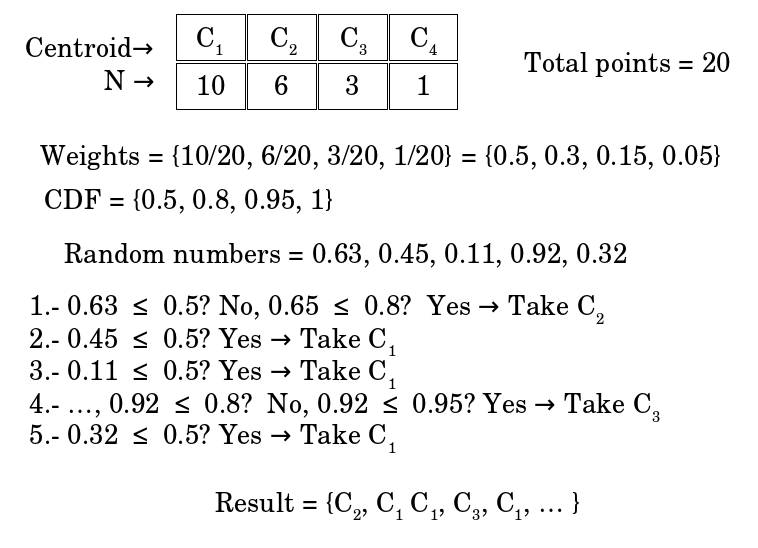
\includegraphics[scale=0.4]{./styles/sampling.png}
 % approxmlast.png: 0x0 pixel, 300dpi, 0.00x0.00 cm, bb=
 \caption{Demonstration: sampling the centroids from weights}
 \label{fig:sampling}
\end{figure}


